% Summary sys_impl here
The core of this system research thesis resides in the system implementation section which answers RQ1. The development will be carried out following an iterative development approach.

This section details the method and the principles that will be used to carry out the software development process of adding support for \gls{HDFS} and \gls{HopsFS} to the delta-rs library.

\subsection{Development process}
The development process will follow an iterative development approach described in Figure \ref{fig:DevProcessRQ1}. 

The first activity will consist of identifying the system requirements and implementation issues collaboratively with the industrial supervisor, who is knowledgeable on Hopsworks' infrastructure (in particular \gls{HopsFS}). Then an iterative loop will start, comprised of an in-depth study of the system and its dependencies, a software design and implementation phase, followed by tests conducted on both the implemented library and its system interactions. This loop will be iterated each time an individual test or an integration test will fail, and for each part of the system until the whole pipeline (from the Python interface to writing on \gls{HopsFS}) will be working as expected. 

Each step of this process is related to one of the goals (G1--G4) associated with RQ1 in Section \ref{sec:goals}. This process will produce a final deliverable (D1), which is a Python wheel of the delta-rs library containing the support for \gls{HDFS} and \gls{HopsFS}.

\begin{figure}[!ht]
    \begin{center}
      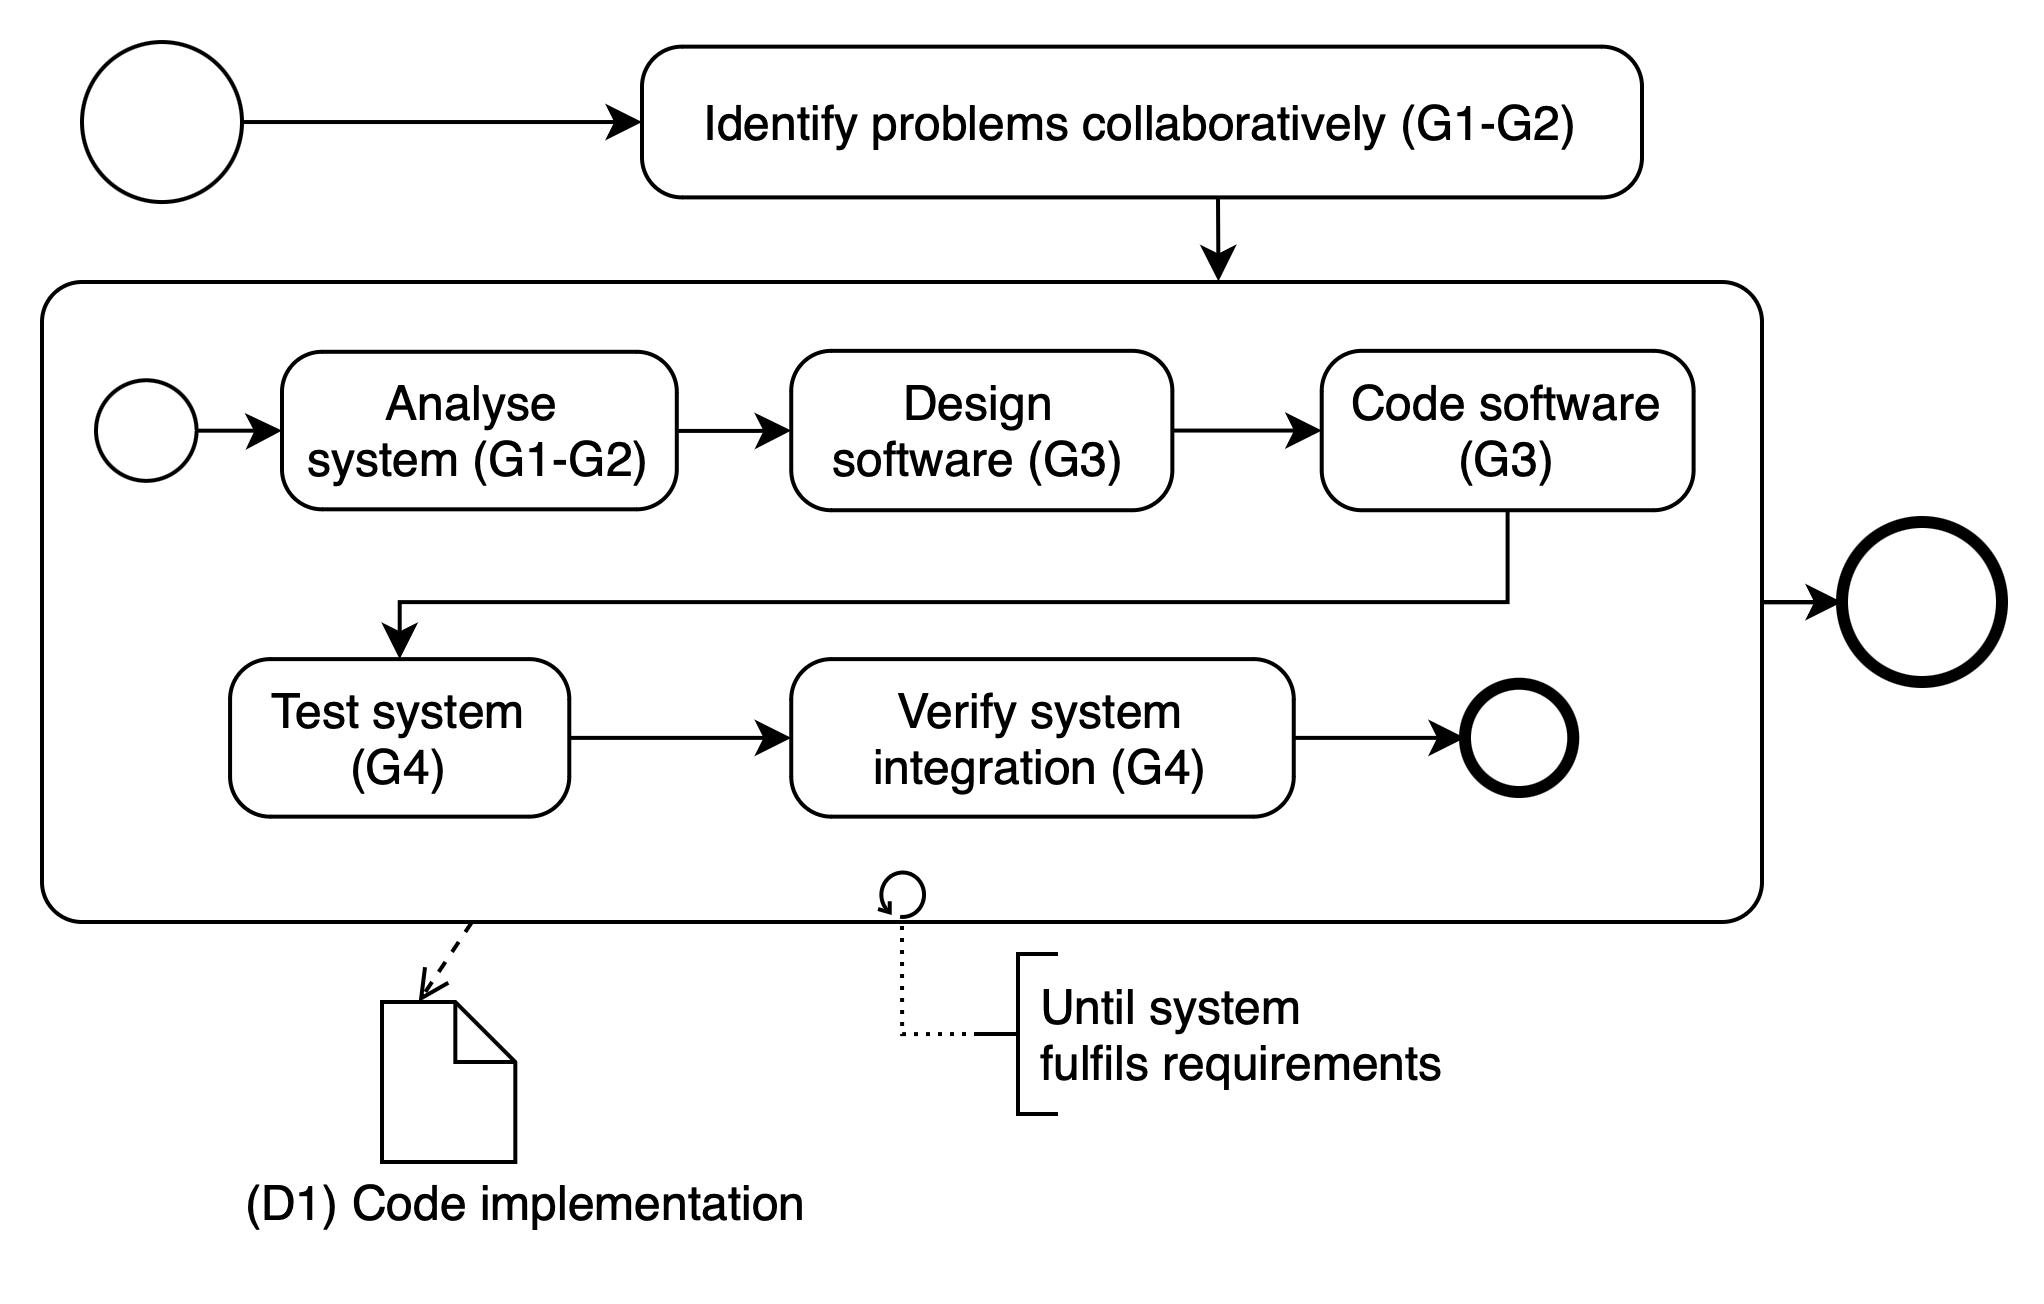
\includegraphics[width=\textwidth]{figures/3-method/research_process_rq1.png}
    \caption{\gls{BPMN} diagram of the System implementation process answering to RQ1. Each activity is associated with a specific Goal (\gls{G}). The process produces a deliverable (\gls{D}), in this case, a code implementation.}
    \label{fig:DevProcessRQ1}
    \end{center}
\end{figure}

\subsection{Requirements}
In the first steps of the system analysis, a series of requirements are defined in agreement with the industrial partner Hopsworks AB, to favor the creation of a solution that could be later used within the company, in a production environment. These are divided into two categories: functional and non-functional requirements. \\ The \textbf{functional requirements} are:
\begin{enumerate}
    \item \textbf{Write Delta Tables}: the solution should allow to write Delta Lake tables on \gls{HopsFS} via the delta-rs library.
    \item \textbf{Read Delta Tables}: the solution should allow to read Delta Lake tables on \gls{HopsFS} via the delta-rs library.
    \item \textbf{Communicate via TLS}: the solution should interact with \gls{HopsFS} via \gls{TLS} protocol version 1.2.
\end{enumerate}
The \textbf{non-functional requirements} are:
\begin{enumerate}
    \item \textbf{Consistent}: the solution should be consistent with the current open-source codebase used when appropriate.
    \item \textbf{Maintainable}: the solution should minimize the need for maintenance and support of the codebase in the future, minimizing changes to open-source code. When appropriate, the changes the solution introduces should be compatible with a future upstream merge to the open-source project modified.
    \item \textbf{Scalable}: the solution should be able to handle larger quantities of data (up to 100 GB) read or written on Delta Tables.
\end{enumerate}

\subsection{Development environment}
The system implementation will be developed by making use of several technologies, here categorized:
\begin{itemize}
    \item \textbf{Computing resources}: the system implementation will be developed in a remote environment accessed via \gls{SSH} from a computer terminal. This remote \gls{VM} is selected as mounting \gls{HopsFS} on a local machine is non-trivial and developing locally could result in inconsistencies when the solution is reproduced in a virtual environment.
    \item \textbf{Writing code}: the Vim \cite{WelcomeHomeVim} text editor is development tool of choice in combination with \gls{CoC} \cite{NeoclideCocnvim2024} providing language-aware autocompletion and rust-analyzer \cite{fannFannheywardCocrustanalyzer2024} access for on-code compiler errors. 
    \item \textbf{Libraries and dependencies}: for simpler development and tests reproducibility, the environment will be set in a Docker container \cite{DockerBuild0200}.
    \item \textbf{Code versioning and shared development}: GitHub \cite{GitHub} will be used for versioning, collaborating with open-source projects (e.g. delta-rs), and sharing the developed solution.
\end{itemize}

 